\documentclass[a4paper]{article}

\usepackage{hyperref}

\usepackage{natbib}
\bibliographystyle{apalike}
\usepackage{graphicx}

\begin{document}

\title{Preferential flow in Daisy 2D\\
  Concept and model for tile drained soil} 
\author{Per Abrahamsen}

\maketitle

This note describes briefly the concept, math, and code behind the
support in Daisy for estimating drain flow dynamics, as well as the
transport of particles and pesticides to tile drains in agricultural
fields.  See \citet{daisy-def,daisy-ems,daisy-new,daisyN} for more
general descriptions of Daisy.

\section{Conceptual model}

The conceptual model is illustrated on figure~\ref{fig:concept}.  In
this section we will discuss the elements of the model in some more
detail.

\begin{figure}[htbp]
  %% trim=l b r t
  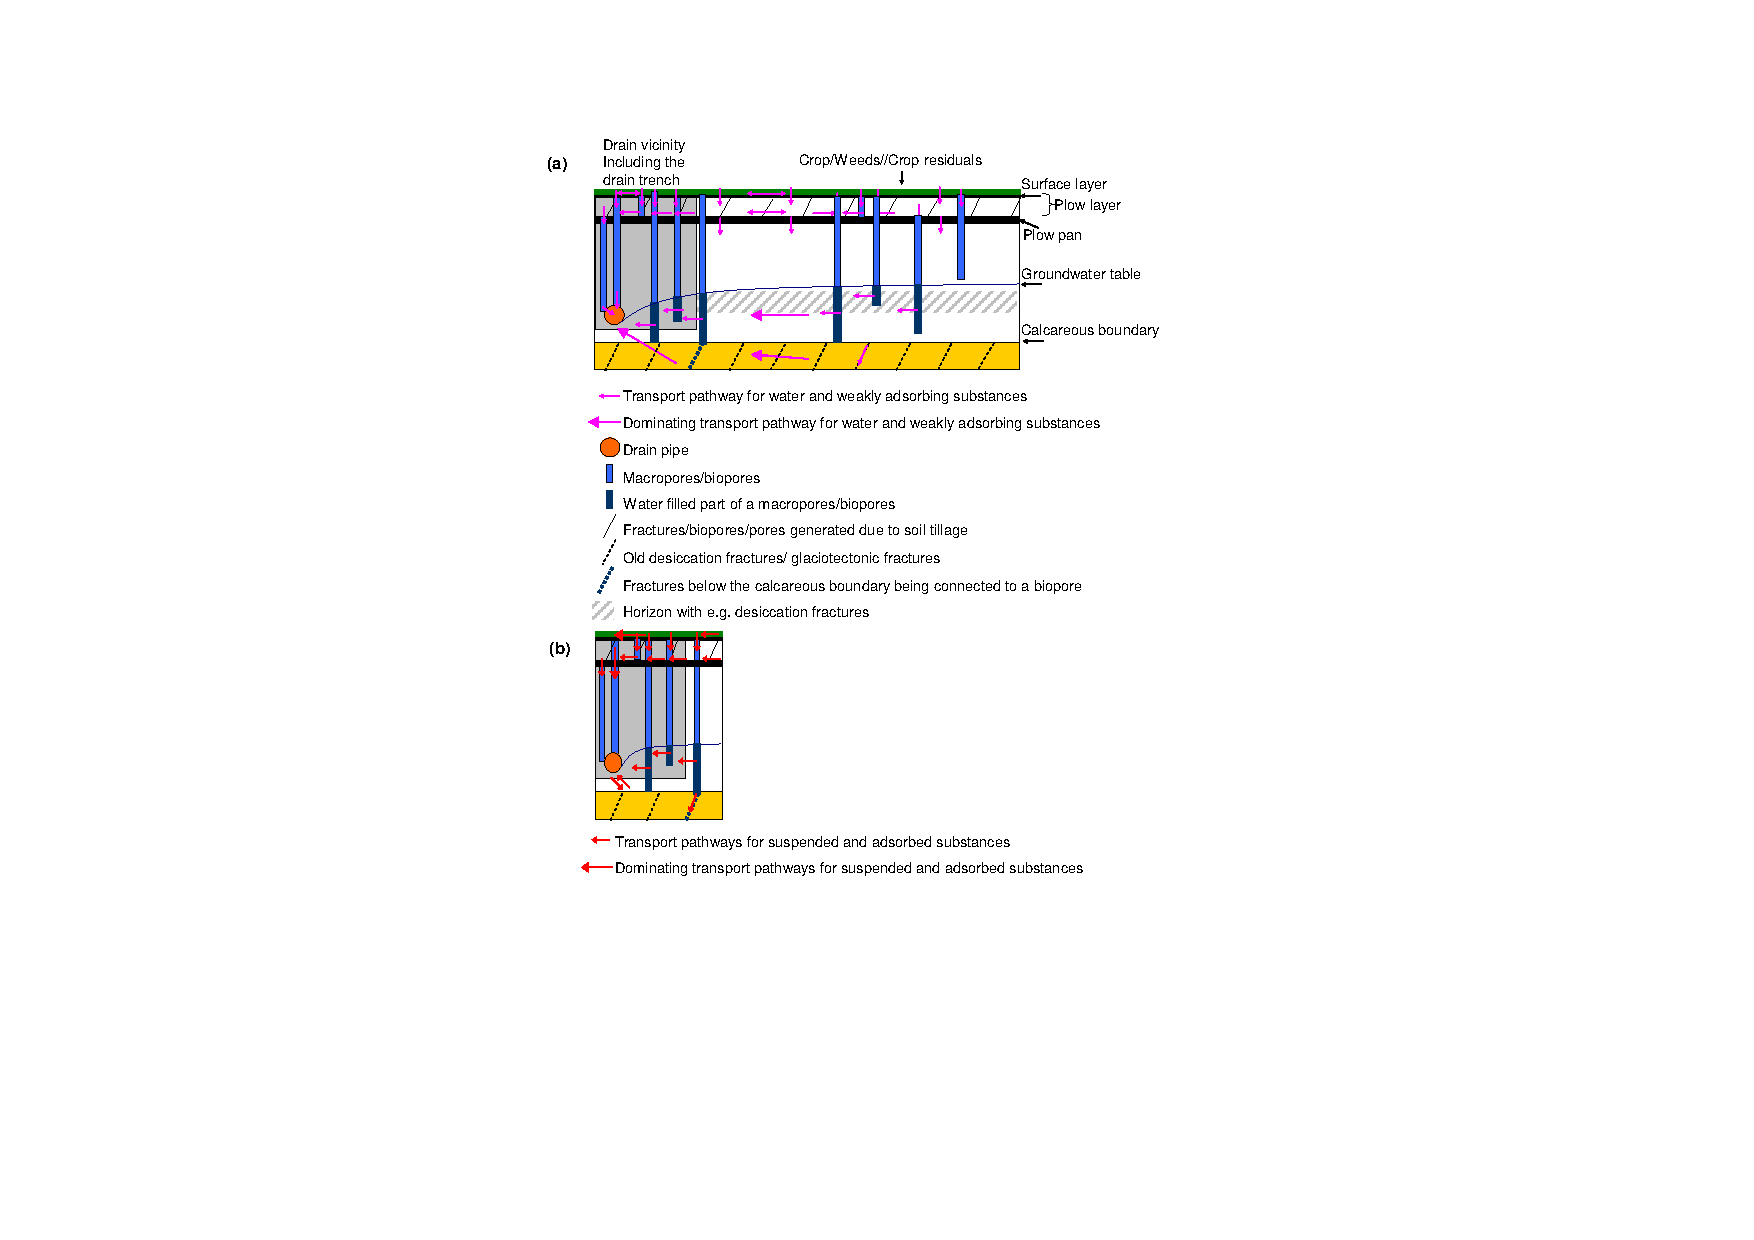
\includegraphics[trim=9cm 6cm 10cm 2cm,clip=true,width=\textwidth]{r2d2-concept}
  \caption{Conceptual model of important structure elements in a
    situation with saturation at drain depth. The model include
    indications of transport pathways (a): for water and weakly
    adsorbing substances and (b): for suspended and strongly adsorbing
    substances.}
  \label{fig:concept}
\end{figure}

\subsection{Soil}

We start with a description of the soil.  The soil is divided into a
number of zones which are considered homogeneous and static with
regard to certain physical attributes, most significantly the soil
texture.  The main division is the horizons, typically with an Ap
horizon (the plowing layer) at top, and a number of other horizons
below.  The top of the Ap horizon is given special regard, the
hydraulic properties will be very dynamic depending on tillage and
weather effects.  The hydraulic properties for the rest of the Ap
horizon will also wary with tillage, but that is not considered.  The
top of the second horizon is also given special regard, as it will
often form a dense plow pan with low hydraulic conductivity.  Finally,
we have a non-horizontal zone, namely the drain trench, which was
formed when the drain tiles were installed.

\subsection{Water flow pathways}

Starting with the smallest water flow pathways, we have the pathways
within the soil aggregates.  These have very limited flow capacity,
but play an important role during spring and summer, as the main
pathways for moving water towards the roots and the soil surface for
transpiration and surface evaporation.  Next step up in size is the
pathways between soil aggregates, in particular soil cracks of various
origins, as they provide a continuous path through the soil.  We only
consider cracks small enough for the capillary forces to have an
effect.  The cracks can potentially have a much higher flow capacity,
but are only activated at near saturated conditions.  Cracks are
characterized by aperture, density, orientation, and location in soil.
The largest pathways considered are earth worm burrows.  These are
large enough that capillary forces no longer play a role, and have a
very high flow capacity, but must be initiated by locally saturated
conditions, and are mostly limited to vertical flow.  Finally we
consider old root channels.  These will largely overlap with the
cracks (for the smaller root channels) and earth worm burrows (for the
larger root channels).  Together, large root channels and earth worm
burrows are referred to as biopores.

The main limitation for flow through biopores is the speed at which
the water can enter or leave.  The biopores may start from the soil
surface, or end in the drain tiles, or in a system of root channels
and cracks that is well connected to the drains.  In the first case,
the flow capacity of water into the biopores from the surface is very
high, in the second case the flow capacity of water out of the
biopores to the drain tiles is very high.  For this reason, biopores
that start at the surface and are well connected to the drain tiles
are of particular importance.  Biopores are characterized by size,
density, location in soil, and whether or not they are connected to
drain pipes.

The biopores will typically be activated when saturated soil is
located above unsaturated soil.  This will (again, typically) happen
at the border between two horizons.  In that respect, the surface and
plow pan are of particular interest.  If a rain event has a low
intensity, the water will enter the soil through the pathways within
and between soil aggregates.  If the rain intensity is higher than the
flow capacity of these pathways, the water will accumulate in the
surface, and once a certain roughness threshold is reached, move
horizontally towards the nearest biopore connected to the surface.  We
ignore the situation where a rain drop falls directly upon a biopore.
If the rain intensity is higher than the flow capacity of water out of
the biopore, water will begin to build up within the biopore, which
will increase the rate of water leaving the biopore.  Once the biopore
is full, water will start accumulating on the surface again, and once
another roughness threshold is reached, move further away towards
biopores that have a better flow capacity of water out of the
biopores.  Something similar may happen on top of the plow pan.  Once
the soil at the bottom of the plowing layer is saturated, biopores
that penetrate the plow pan will be activated, and water will move
through the soil toward these biopores.  And again, when the local
biopores are filled, water may start moving towards the drain
connected biopores.  The same can happen elsewhere in the soil, but
the surface and plow pan are considered the two most important
barriers.  Once a biopores has become activated, it may continue to
extract water from the surrounding soil through connected film flow
inside the biopores, until the soil becomes too dry, as demonstrated
in \citet{tofteng2002film,gjettermann2004transport}.

As described above, drain flow can occur whenever the biopores are
activated, that is when we have localized saturated conditions above
the drain pipes.  The drain season is when we have saturated
conditions at drain depth.  Between drains we may have saturated
conditions above drain depth.  This pressure potential will cause a
horizontal flow towards the drain pipes, mostly through the flow
pathways that goes between soil aggregates, in particular cracks.

\subsection{Colloids and pesticide transport}

Chemicals (such as pesticides) dissolved into the water mostly follows
the flow of the water, with the addition of diffusion between water
with different concentrations, which is a relatively slow process
compared to advection.  In Daisy, we ignore diffusion in cracks and in
biopores.  However, of particular interest here is diffusion between
water in cracks and water inside soil aggregates.  Depending on the
timing, this might cause water with a high solute concentration to
bypass soil volumes with relatively clean water, or allow solutes to
be protected within the soil aggregates while relatively clean water
pass by in the cracks and biopores.

Chemicals that are sorbed to soil particles move together with the
soil particles, which is to say, mostly not at all.  However, soil
particles may be released by various means, of which only one is
considered in the model: Clay particles released as a result of the
impact of rain drops on the soil surface.  As the particles are large,
they will tend to be filtered quickly if they enter soil aggregates,
less quickly when moving between soil aggregates, and not at all when
moving within biopores.  Chemicals are thus generally found in three
forms in the soil.  Dissolved, sorbed to immobile soil, and sorbed to
mobile soil particles.  

\section{Mathematical model}

In Daisy, the flow pathways within soil aggregates are referred to as
the primary domain.  The flow pathways between soil aggregates,
including cracks, are referred to as the secondary domain.  Together
these two domains where the capillary forces are active is called the
matrix domain.  The large biopores where the capillary forces no
longer are significant constitute the tertiary domain.

The mathematical model for 2D water flow and solute transport is
described in~\citet{mollerup2011,SAFIRD32,daisy2Ddnumerics} with
increasing level of details.  The model behind colloid generation and
filtration can mostly be found in~\citet{macro-colloid}.

\section{Software model}

The Daisy tutorial \citep{daisy-tut} describes how to set up Daisy for
a one dimensional column.  In this section we will give an overview of
how the new features discussed in this paper are specified. A complete
reference can be found in \citet{daisy-ref}.

\subsection{Soil}

Assume we already have defined three horizons, ``Ap'', ``B'', and
``C''.  We can then use these to define the surface and plow pan by
adjusting the hydraulic conductivity and bulk density.
\begin{verbatim}
  (defhorizon "Surface" "Ap"
    (hydraulic original (K_sat 0.17 [cm/h])))

  (defhorizon "Plow pan" "B"
    (dry_bulk_density 1.70 [g/cm^3])
    (hydraulic original (K_sat 0.04 [cm/h])))
\end{verbatim}
If no better information exists, leave the surface unchanged and set
the saturated hydraulic conductivity of the plow pan to 10\% of the
value for the B horizon.

If we want a dynamic surface horizon, it become more complicated.  The
\verb|M_vG_compact| hydraulic model allows the Mualem -- van Genuchten
parameters to be a function of the porosity ($\Theta_{\mbox{sat}}$ or
\verb|Theta_sat|).  For example, the van Genuchten $n$ parameter is
calculated as $n = n_{\mbox{ref}} \times n_{\mbox{mod}}
(\Theta_{\mbox{sat}})$.  $n_{\mbox{mod}}$ is specified as a
piecewise linear function defined by number of points of the form
($\Theta_{\mbox{sat}}$ \emph{value}).
\begin{verbatim}
  (defhorizon Surface Ap
    (hydraulic M_vG_compact
               (Theta_res 0 [%])
               (Theta_sat 0.39 [])
               (ref_alpha 0.01 [cm^-1])
               (ref_n 1.1 []) 
               (ref_K_sat 2.25 [cm/h])
               (mod_alpha (0 1) (1 1))
               (mod_n  (0 1) (1 1))
               (mod_K_sat  (0.3 0.001) (0.35 0.01) (0.39 1))))
\end{verbatim}
In this example, \verb|K_sat| is decreased to 1\% when
\verb|Theta_sat| is decreased to 35\%, and decreased to 0.1\% when
\verb|Theta_sat| is decreased to 30\%.  You can set the porosity with
a pseudo-manager operation.
\begin{verbatim}
  (wait (at 2000 06 01))
  (set_porosity (depth -1 [cm]) (porosity 0.35))
\end{verbatim}
In general, you should decrease the porosity after the first rain
event, and reset it to the normal level after tillage.  The new
pseudo-horizons are specified like the normal horizons.

The drain trench is defined the same way as you specify a normal
horizon.  However, since it partly overlap with the horizons is
enabled differently, based on both horizontal and vertical limits.
\begin{verbatim}
  (Soil (MaxRootingDepth 150 [cm])
        (horizons (-3.00 "Surface")
                  (-25.00 "Ap")
                  (-33.00 "Plow pan")
                  (-120 "B")
                  (-200 "C"))
        (zones ((box (top finite -33 [cm]) (bottom finite -120 [cm])
                     (left finite  0 [cm]) (right finite    25 [cm]))
                "Drain trench")))
\end{verbatim}

\subsection{Cracks and pathways between soil aggregates}

Daisy can handle three different situation with regard to cracks and
pathways between soil aggregates (collectively referred as the
secondary domain).  The first is the simplest, there are no cracks.
We then use pressure head to specify the border between the primary
domain (pathways within soil aggregates) and the secondary domain
($h_{\mbox{lim}}$).  We also specify an exchange rate for solutes
between the primary and secondary domain ($\alpha$).
\begin{verbatim}
  (defsecondary no_cracks pressure 
    (alpha 0.001 [h^-1]))  
    (h_lim 2 [pF]))

  (defhorizon Ap ;; More ...
    (secondary no_cracks))
\end{verbatim}

The second option is that we have cracks with no particular
orientation (vertical or horizontal).  In that case effective aperture
and density of the cracks, along with $\alpha$ as before.  The
aperture will form the basis of the division between the domains, and
together with density is will also be used for calculating the
hydraulic conductivity within the secondary domain.
\begin{verbatim}
  (defsecondary has_cracks cracks
    (aperture 78 [um])
    (density 10 [m^-1])
    (alpha 0.001 [h^-1]))

  (defhorizon B ;; More ...
    (secondary has_cracks))
\end{verbatim}

The third option is that we have cracks with a clear horizontal or
vertical orientation.  In that case, we use the vertical conductivity
as basis, and specify the horizontal conductivity through the
\verb|anisotropy| horizon parameter.  The anisotropy parameter affects
both conductivity in the primary and the secondary domain, but
significant horizontal water movement is only expected in saturated or
near saturated conditions, where the secondary domain will dominate.
\begin{verbatim}
  (defhorizon C ;; More ...
    (secondary no_cracks)
    (anisotropy 12))
\end{verbatim}
If the cracks are vertical, you may want to use a bimodal hydraulic
model, such as \verb|M_BaC_Bimodal| or \verb|M_vGp| \citep{MvGp}.

\subsection{Biopores}

The biopores are divided into classes with common properties.  The
properties are where they start, where they end, their diameter, and
whether they are well connected to drains.  For biopores well
connected to drains we also need to know the position of the drains.
For biopores that are not well connected to the drains, we need to
know the hydraulic conductivity of the biopore wall.  The conductivity
is specified relative to the surrounding soil matrix, and the
thickness of the wall is assumed to be 10\% of the diameter.  We also
specify the density, as a function of distance to drain ($x$).

In the following we define three biopore classes.  The first class
consist of short, narrow biopores, going from the soil surface to the
borrom of the plowing layer.  This class is uniformly distributed.
The next two classes are long wide biopores that start at the soil
surface and go down to 1.25 meter below.  The biopores less than
approximately 25 cm from the drain are considered well connected to
the drains.  The rest are not.  Finally we define a tertiary domain
consisting of these three classes, and name it ``MyBiopores''.  There
is no limit to the number of biopore classes you can have, but
simulation time will suffer if you have too many, and there is an
increased risk of instability.
\begin{verbatim}
  (defbiopore "short"
    (matrix (height_start 0 [cm])
            (height_end -25 [cm])
            (diameter 2 [mm])
            (density 100 [m^-2])
            (K_wall_relative 1 [%])))

  (defbiopore "long"
    (matrix (height_start  0 [cm])
            (height_end -125 [cm])
            (density 10 [m^-2])
            (diameter 4 [mm])
            (density (plf x (range [m^-2])
                            (domain [cm])
                            (points (20 0) (30 15))))
            (K_wall_relative 1 [%])))

  (defbiopore "connected"
    (drain (height_start  0 [cm])
           (height_end -125 [cm])
           (diameter 4 [mm])
           (density (plf x (range [m^-2])
                           (domain [cm])
                           (points (20 15) (30 0))))
           (pipe_position -110 [cm])))

  (deftertiary MyBiopores biopores
    (classes ("short") ("long") ("connected")))
\end{verbatim}

\subsection{2D movement}

The \texttt{Movement} parameter is where is where you specify the
geometry and enable the biopores.  The \texttt{rectangle} movement
model provides a 2D grid where you specify the endpoints with
\texttt{zplus} and \texttt{xplus}.  You also specify the location of
the drain here, depth first.  And finally, this is where you enable
the tertiary domain.
\begin{verbatim}
  (Movement rectangle
    (Geometry (zplus -1.5 -3 -5.5 -10 -14 -18 -22 -25 
                     -27 -30 -33 -40 -50 -60 -75 -90 -100 -120
                     -125 -150 -170 -200 [cm])
              (xplus 25 50 100 150 300 500 650 800 [cm]))
    (drainpoints (-110.0 [cm] 1 [cm]))
    (Tertiary MyBiopores))
\end{verbatim}
This is also where you specify the numeric details of the transport
algorithms, which can be important for stability.

\subsection{Colloids and pesticides}

In Daisy terminology, a ``chemistry'' refers to a collection of
substances and reactions.  A ``chemical'' is just a name of for a
something that can be tracked by Daisy, in the following we define
``chemicals'' that to track different forms of the same chemical.  For
colloids, we just define one substance (colloids) and two reactions
(generation and filtration).

\begin{verbatim}
  (defchemical colloid common
    "Mobile colloids."
    (diffusion_coefficient 4.6e-6 [cm^2/s])
    (decompose_rate 0 [h^-1]))
  
  (defreaction colloid-generation colgen_Jarvis99
    "Release of colloids in soil surface from heavy rain."
    (kd 15 [g/J])       ;Detachment rate coefficient.
    (kr 0.05 [g/m^2/h]) ;Replenishment rate coefficient.
    (zi 0.05 [cm])      ;Surface layer thickness.
    (colloid colloid))
  
  (defreaction colloid-filter filter_velocity
    "Filtration of colloids in the soil matrix."
    (fc_primary 80 [m^-1])   ;Filter coefficient primary domain.
    (fc_secondary 40 [m^-1]) ;Ditto for secondary domain.
    (mobile colloid))
  
  (defchemistry colloids default
    (trace colloid)
    (reaction colloid-generation colloid-filter))
\end{verbatim}

For sorbing pesticides, things get more complicated.  The pesticides
move differently depending on whether they are dissolved, or sorbed,
and if sorbed whether they are sorbed to a colloid, or to the soil
matrix.  So they have three forms, dissolved, immobile, and colloid
bound.  We also define a base form from which they are all derived,
and define the decompose rate here (assuming the decompose rate is the
same for all forms). The pesticide can change between all three forms.
The dissolved form can be sorbed or desorbed to either the soil matrix
or colloids.  A \verb|soil_enrichment_factor| parameter determines how
much more likely a colloid is to receive the pesticide compared to an
immobile soil particle.  A $K_{\mbox{oc}}$ or $K_d$ determines the
equilibrium between the sorbed and desorbed forms.  A
\verb|k_sorption|, and if different \verb|k_desorption|, parameter
determine the rate at which equilibrium is reached.  Finally, immobile
pesticides will be transformed to colloid bound pesticides at the same
rate immobile soil particles are transformed into colloids, and
colloid bound pesticides will become immobile at the same rate
colloids are filtered in the soil matrix.

\begin{verbatim}
  (defchemical Pendimethalin-base herbicide
    "Base parameterization for all Pendimethalin forms."
    (decompose_halftime 90 [d]))          ;27-186 [d]
  
  (defchemical Pendimethalin Pendimethalin-base
    "Dissolved pendimethalin."
    (adsorption none))
  
  (defchemical Pendimethalin-immobile Pendimethalin-base
    "Pendimethalin sorbed to immobile soil."
    (adsorption full))
  
  (defreaction Pendimethalin-immobile-sorption sorption
    "Sorption equilibrium between dissolved and immobile Pendimethalin."
    (sorbed Pendimethalin-immobile)
    (solute Pendimethalin)
    (K_OC 15744 [ml/g])                   ;6700-29400 [ml/g]
    (k_sorption 0.05 [h^-1]))
  
  (defchemical Pendimethalin-colloid Pendimethalin-base
    "Pendimethalin sorbed to colloids."
    (adsorption none)
    (diffusion_coefficient 4.6e-6 [cm^2/s]))
  
  (defreaction Pendimethalin-colloid-sorption Pendimethalin-immobile-sorption
    "Sorption equilibrium between dissolved and colloid-bound Pendimethalin."
    (colloid colloid)
    (soil_enrichment_factor 10000 [])
    (sorbed Pendimethalin-colloid)
    (k_sorption 0.05 [h^-1]))
  
  (defreaction Pendimethalin-filter colloid-filter
    "Filtration of colloid-bound pendimethalin in the soil matrix."
    (mobile Pendimethalin-colloid)
    (immobile Pendimethalin-immobile))
  
  (defreaction Pendimethalin-colloid-generation bound_release
    "Release immobile Pendimethalin as colloids in mixing layer."
    (colloid colloid)
    (immobile Pendimethalin-immobile)
    (bound Pendimethalin-colloid))
  
  (defchemistry Pendimethalin default
    "Pendimethalin in both immobile, solute and colloid form."
    (trace Pendimethalin Pendimethalin-immobile Pendimethalin-colloid)
    (reaction Pendimethalin-immobile-sorption
              Pendimethalin-filter 
              Pendimethalin-colloid-generation
              Pendimethalin-colloid-sorption))
\end{verbatim}

The defined chemistries are enabled in the column definition.  You
must list colloids before any pesticides that can be bound to
colloids.  You can list as many pesticides as you want, but simulation
time will increase linearly with the number of pesticides.
\begin{verbatim}
  (Chemistry multi (combine colloids Pendimethalin))
\end{verbatim}

\bibliography{daisy}

\end{document}

%%% Local Variables: 
%%% mode: latex
%%% TeX-master: t
%%% End: 
